\section{Results}
First, we tested the model with the perception data. 
Significance values were determined by using the cumulative binomial distribution to estimate the likelihood of observing a given classification rate by chance \cite{Combrisson2015}. 
Using the cumulative binomial distribution allows us to determine the number of observations that are correctly classified by chance with respect to the number of observations.
Our model was able to classify the 12-classes (12 stimuli listed in \autoref{tab:stimuli_information}) with a 28.7\% accuracy rate (chance = 17.59\%) at a significance level of p=0.001.
\autoref{fig:model_W_confusion} is a confusion matrix which shows the classification results for each stimulus.
\begin{figure}[htb] 
  \begin{center}
    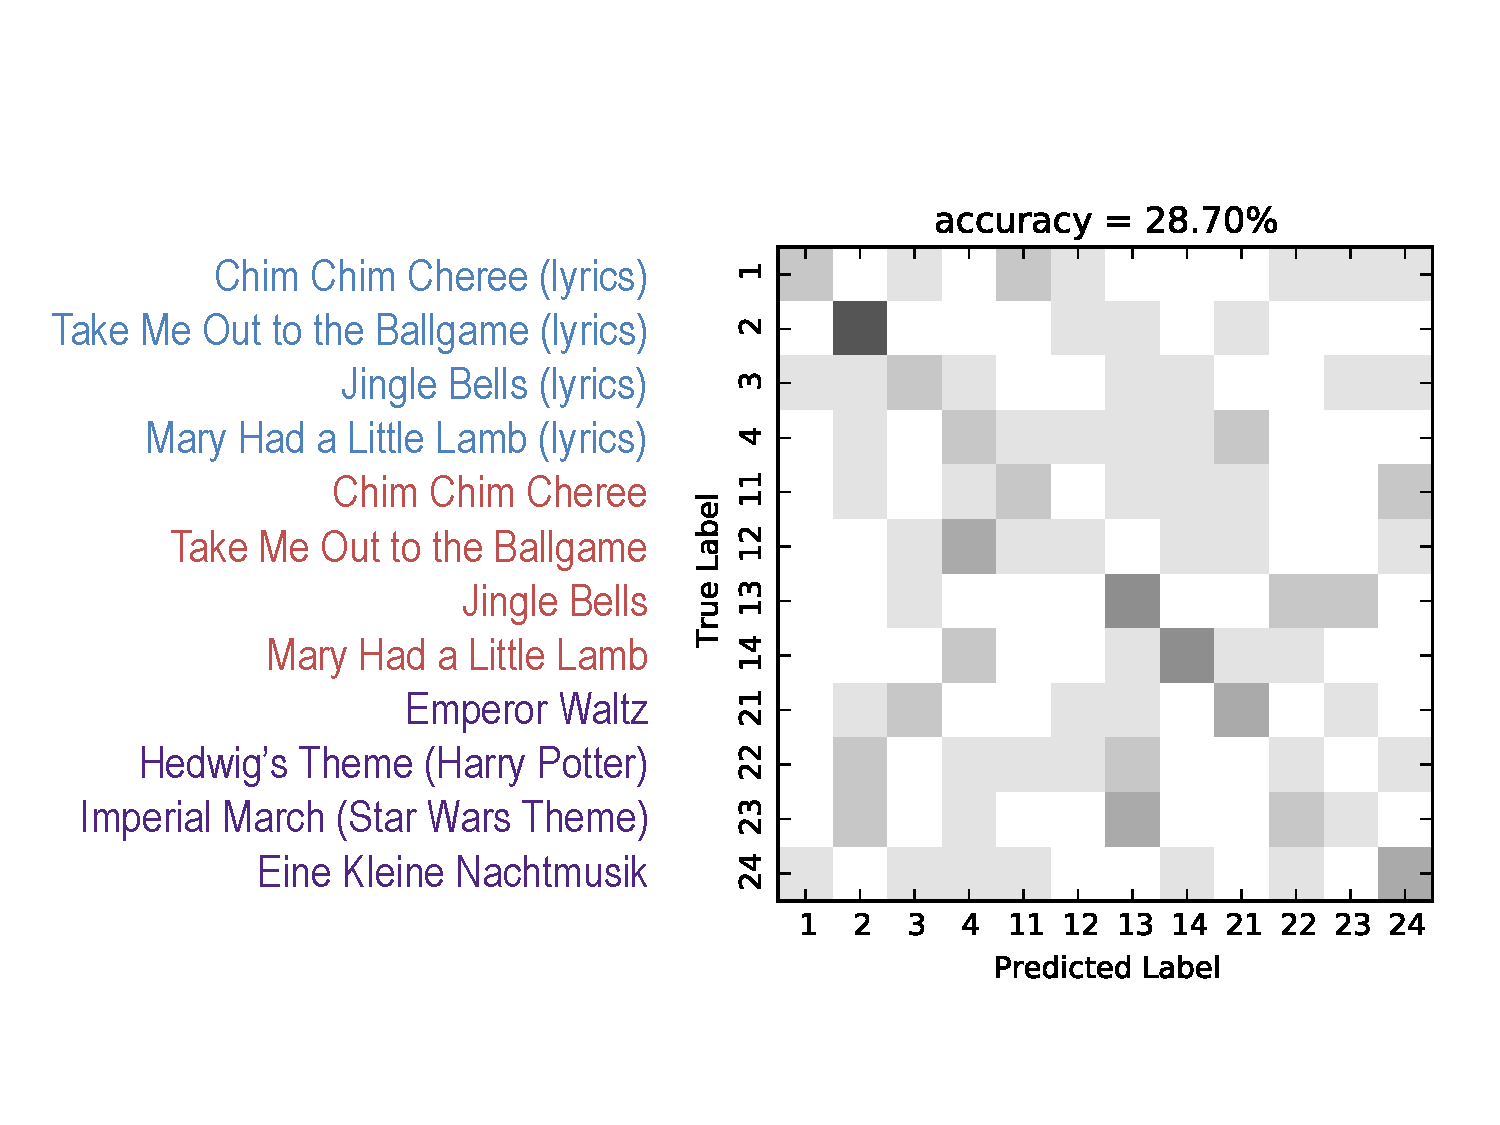
\includegraphics[width=.75\textwidth,keepaspectratio=true]{Figures/model_W_confusion-512}
   \\\vspace{-0.8em}
    \caption{12-class confusion matrix for perception data. The numbers are the ID numbers of the stimuli found in \autoref{tab:stimuli_information}. Colour indicates the number of times a true label was classified as a predicted label with darker colours indicating more classifications.}
    \label{fig:model_W_confusion}
  \end{center}
%  \vspace{-1em}
\end{figure}
From the confusion matrix we can see that some stimuli were more accurately classified than others. 
Stimulus 2 (Take Me Out to the Ballgame with lyrics) is the most accurately classified. 
Stimuli 13 and 14 are also accurately classified, but some confusion with their lyric counterparts (stimuli 3 and 4) can be seen.
Confusion between lyric and non-lyric pairs can also be seen with stimulus 1 being classified as stimulus 11.

To further investigate which pairs of stimuli the classifier could distinguish best, we put all combinations of paired stimuli through our classifier.
This resulted in the series of binary confusion matrices in \autoref{fig:model_W_binary_confusion} that show us that some pairs of stimuli are more easily differentiated than others. 
\begin{figure}[htb] 
  \begin{center}
    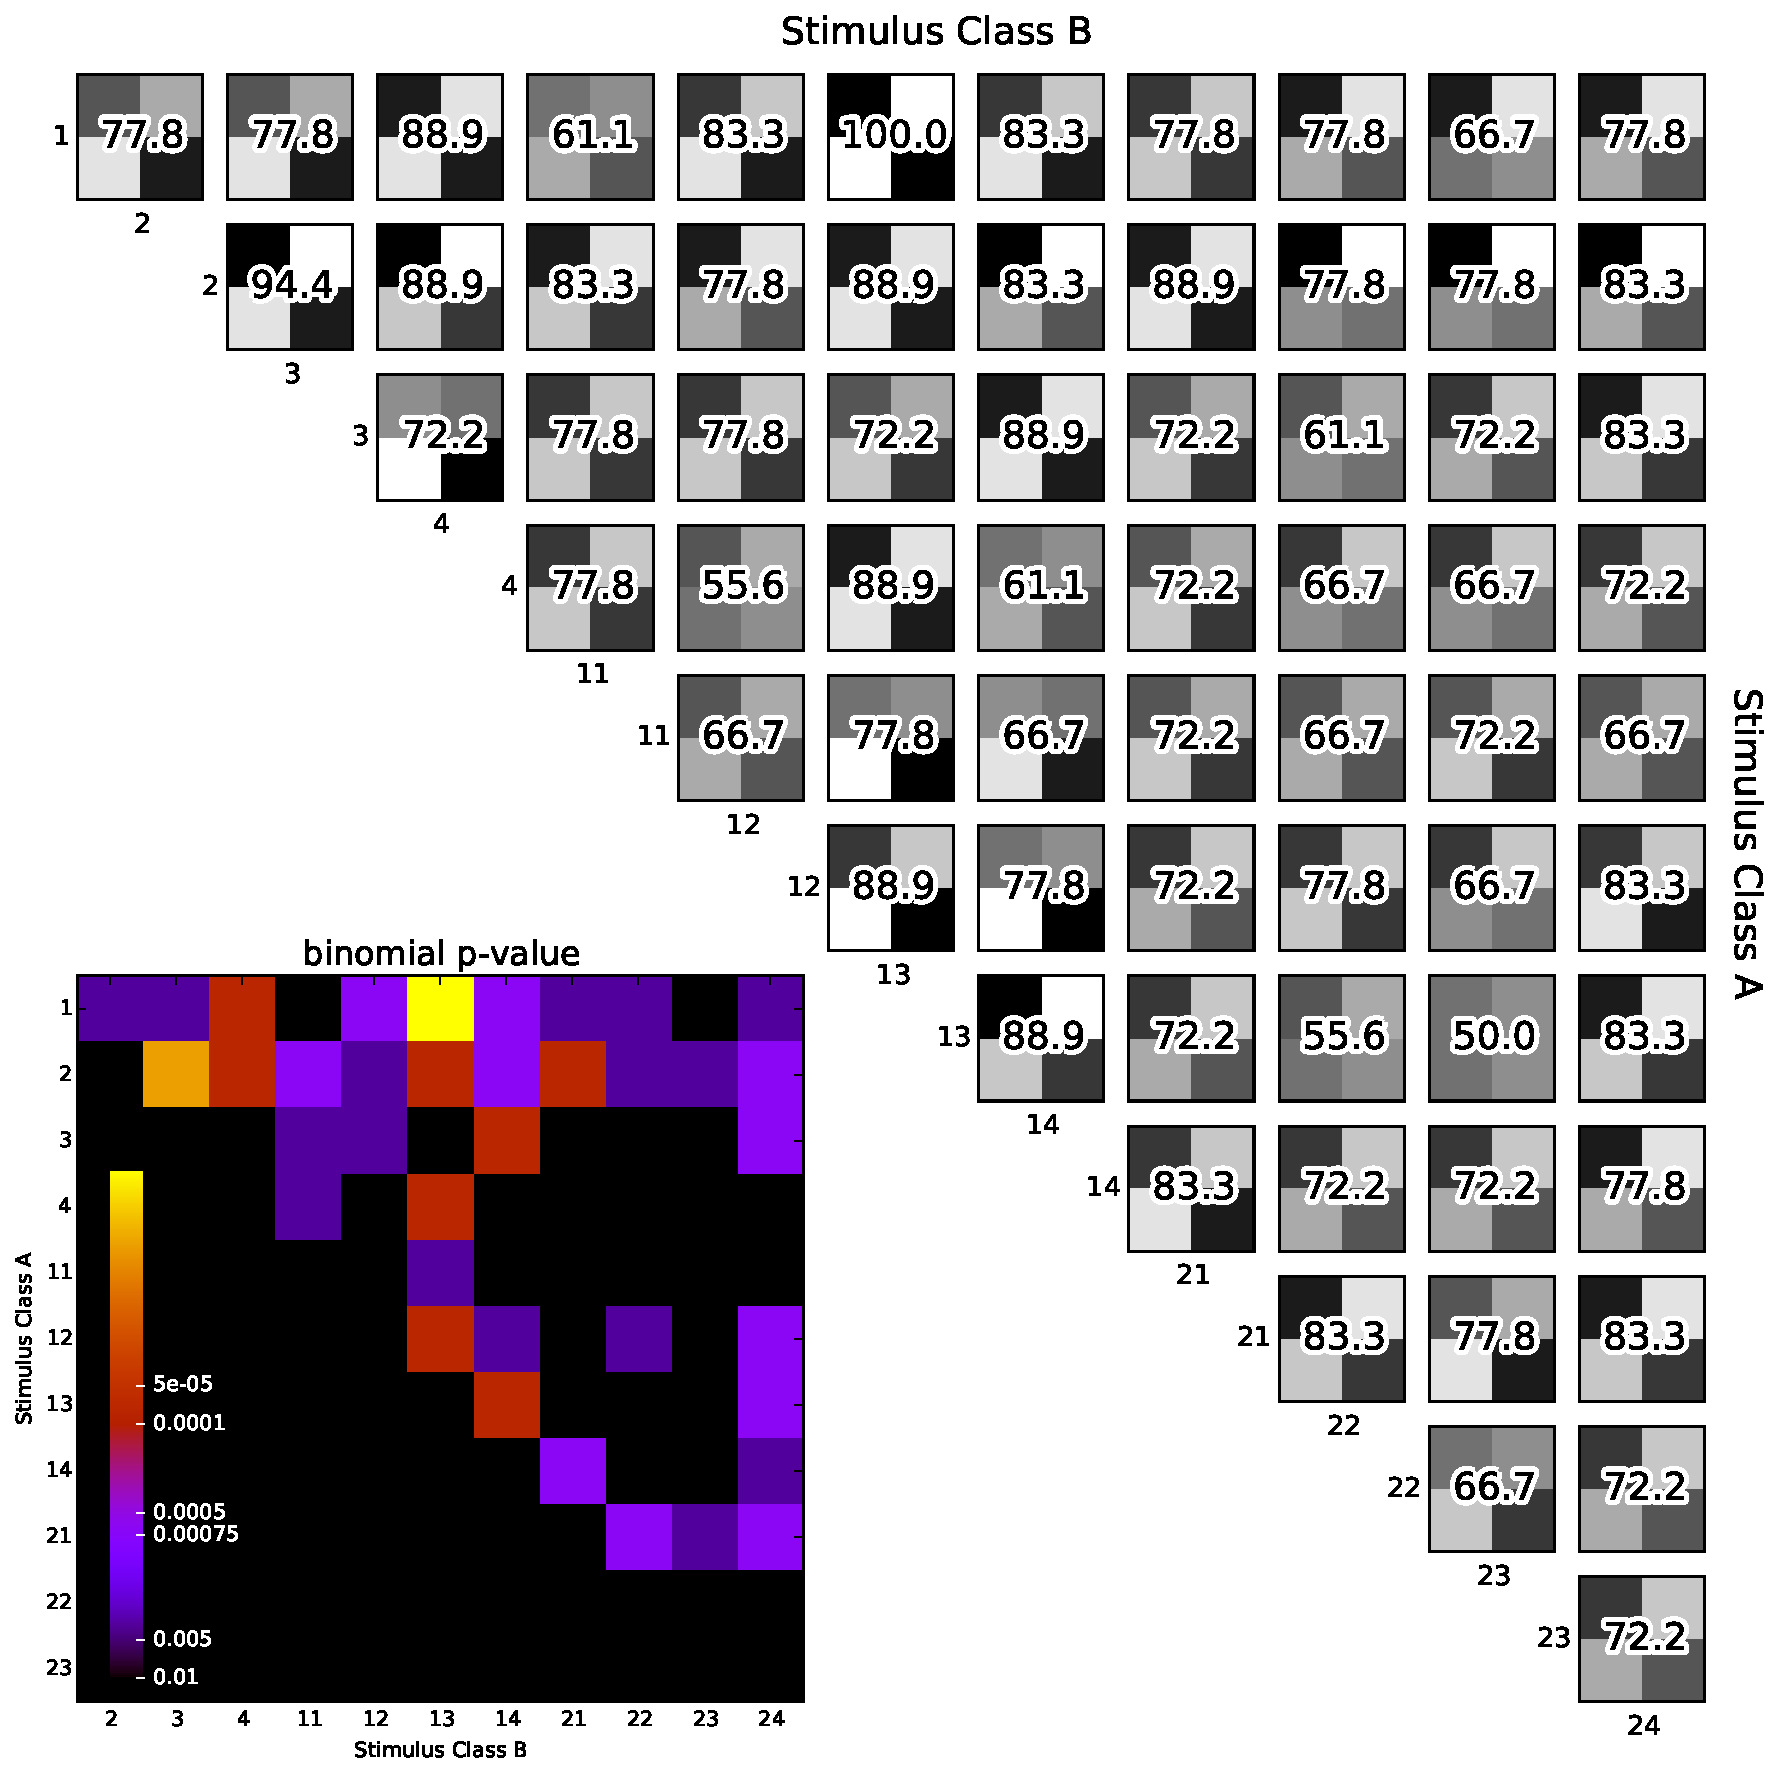
\includegraphics[width=.8\textwidth,keepaspectratio=true]{Figures/model_W_binary_confusion-512}
   \\\vspace{-0.8em}
    \caption{Binary confusion matrices for perception data.
    The inset shows the p-values determined by using the cumulative binomial distribution to estimate the likelihood of observing the respective binary classification rate by chance. The significance threshold was bonferroni corrected to $alpha$ =  0.05/66 = 7.5e-04}
    \label{fig:model_W_binary_confusion}
  \end{center}
  \vspace{-1em}
\end{figure}
For example: Chim Chim Cheree with lyrics is classified correctly 100\% of the time when paired with Jingle Bells without lyrics.
Within each binary confusion matrix chance is 66.67\% (alpha = 0.05).
The statistical significance (p-value) of each of the comparisons is visualized in the figure's inset. 
%Most of the binary comparisons are classified correctly at a statistically significant level (p$<$0.05). 

The imagination data was then tested on the same model (i.e. there was no additional training using the imagination data). 
The model was not able to classify the 12 stimuli from the EEG data collected during music imagination. 
\autoref{fig:model_W_confusion_cond2} is a confusion matrix which shows the imagination classification results at 7.41\% (below chance = 12.96\%, alpha = 0.05). 
As can be seen in the figure, there is no clear pattern to the confusion indicating that the system was not making classification errors in a systematic way. 
\begin{figure}[htb] 
  \begin{center}
    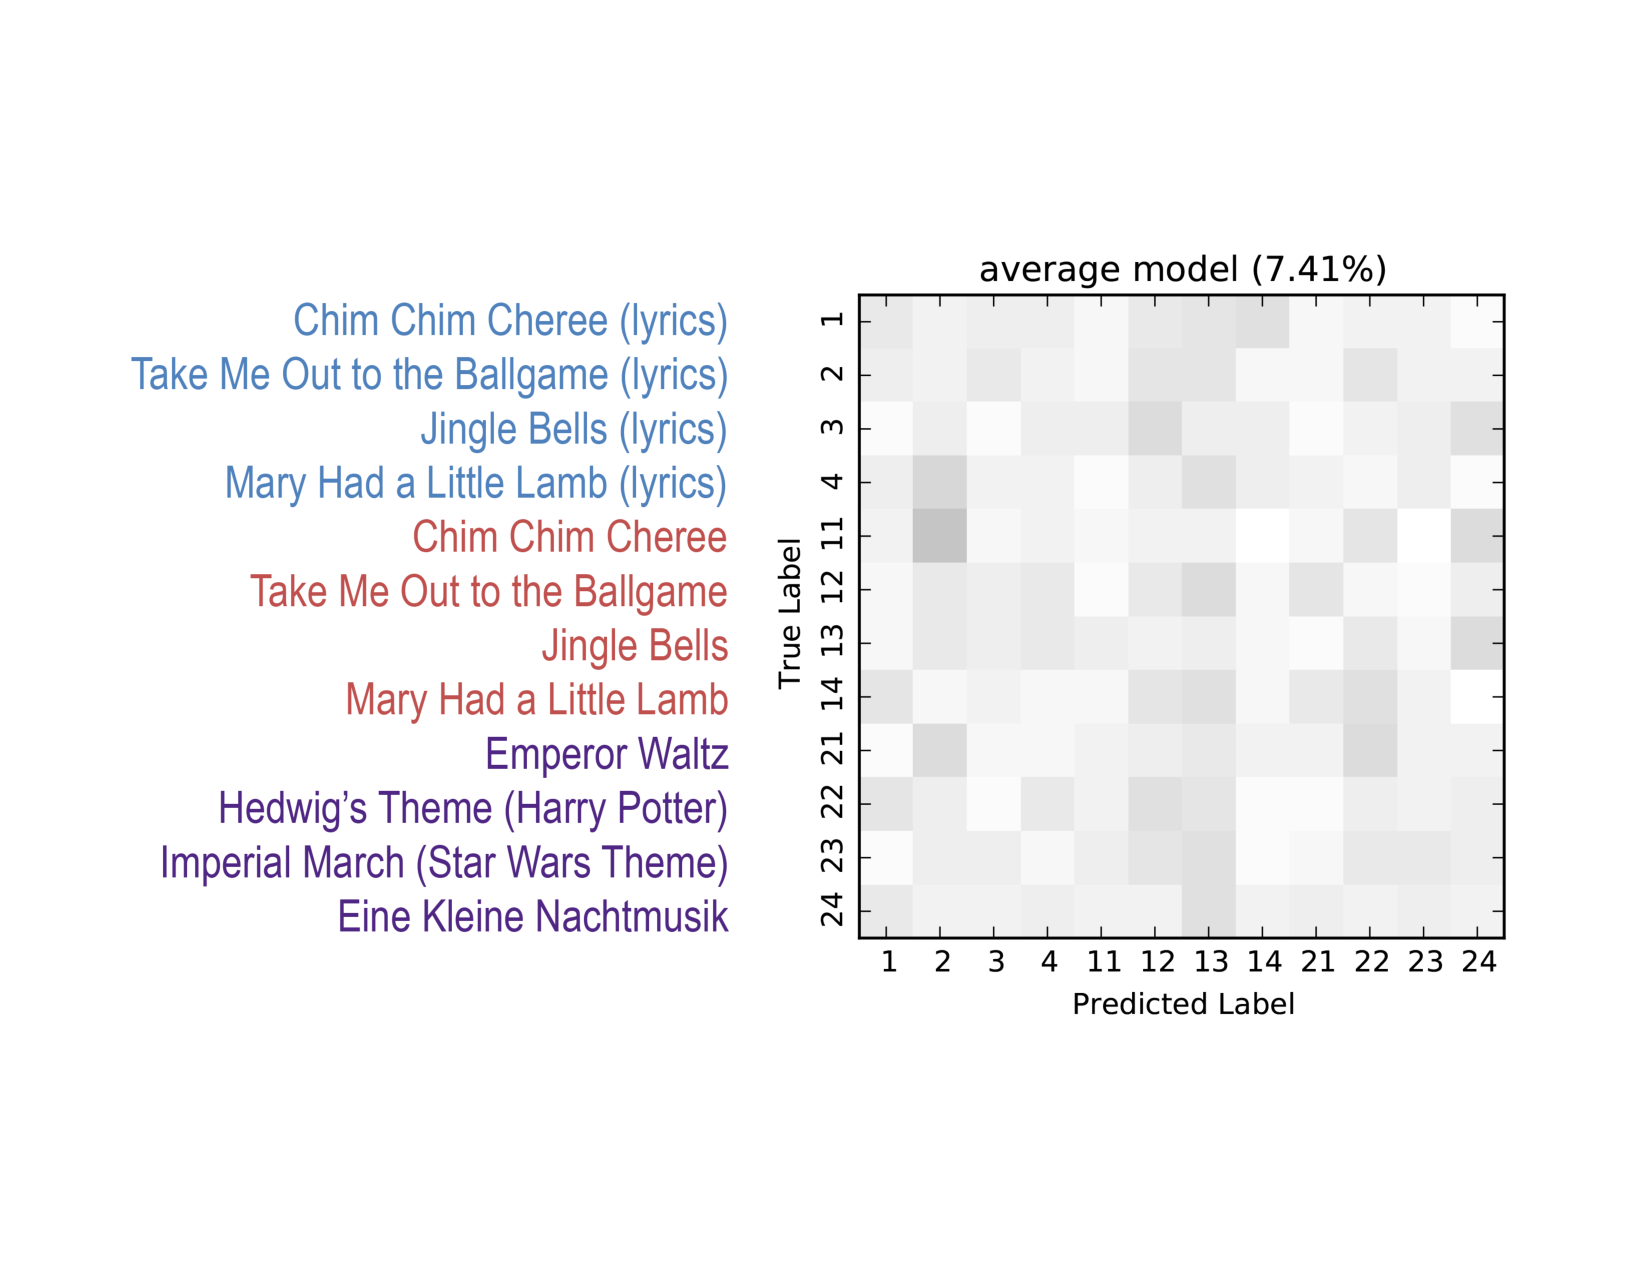
\includegraphics[width=.83\textwidth,keepaspectratio=true]{Figures/model_W_confusion_cond2}
   \\\vspace{-0.8em}
    \caption{12-class confusion matrix for imagination data. The numbers are the ID numbers of the stimuli found in \autoref{tab:stimuli_information}. Colour indicates the number of times a true label was classified as a predicted label with darker colours indicating more classifications.}
        \label{fig:model_W_confusion_cond2}
  \end{center}
  \vspace{-1em}
\end{figure}

We investigated whether there were pairs of imagined stimuli that the classifier could distinguish.
\autoref{fig:model_W_binary_confusion_cond2} shows the binary confusion matrix.
None of the stimulus pairs were classified at a statistically significant level. 

\begin{figure}[h] 
  \begin{center}
    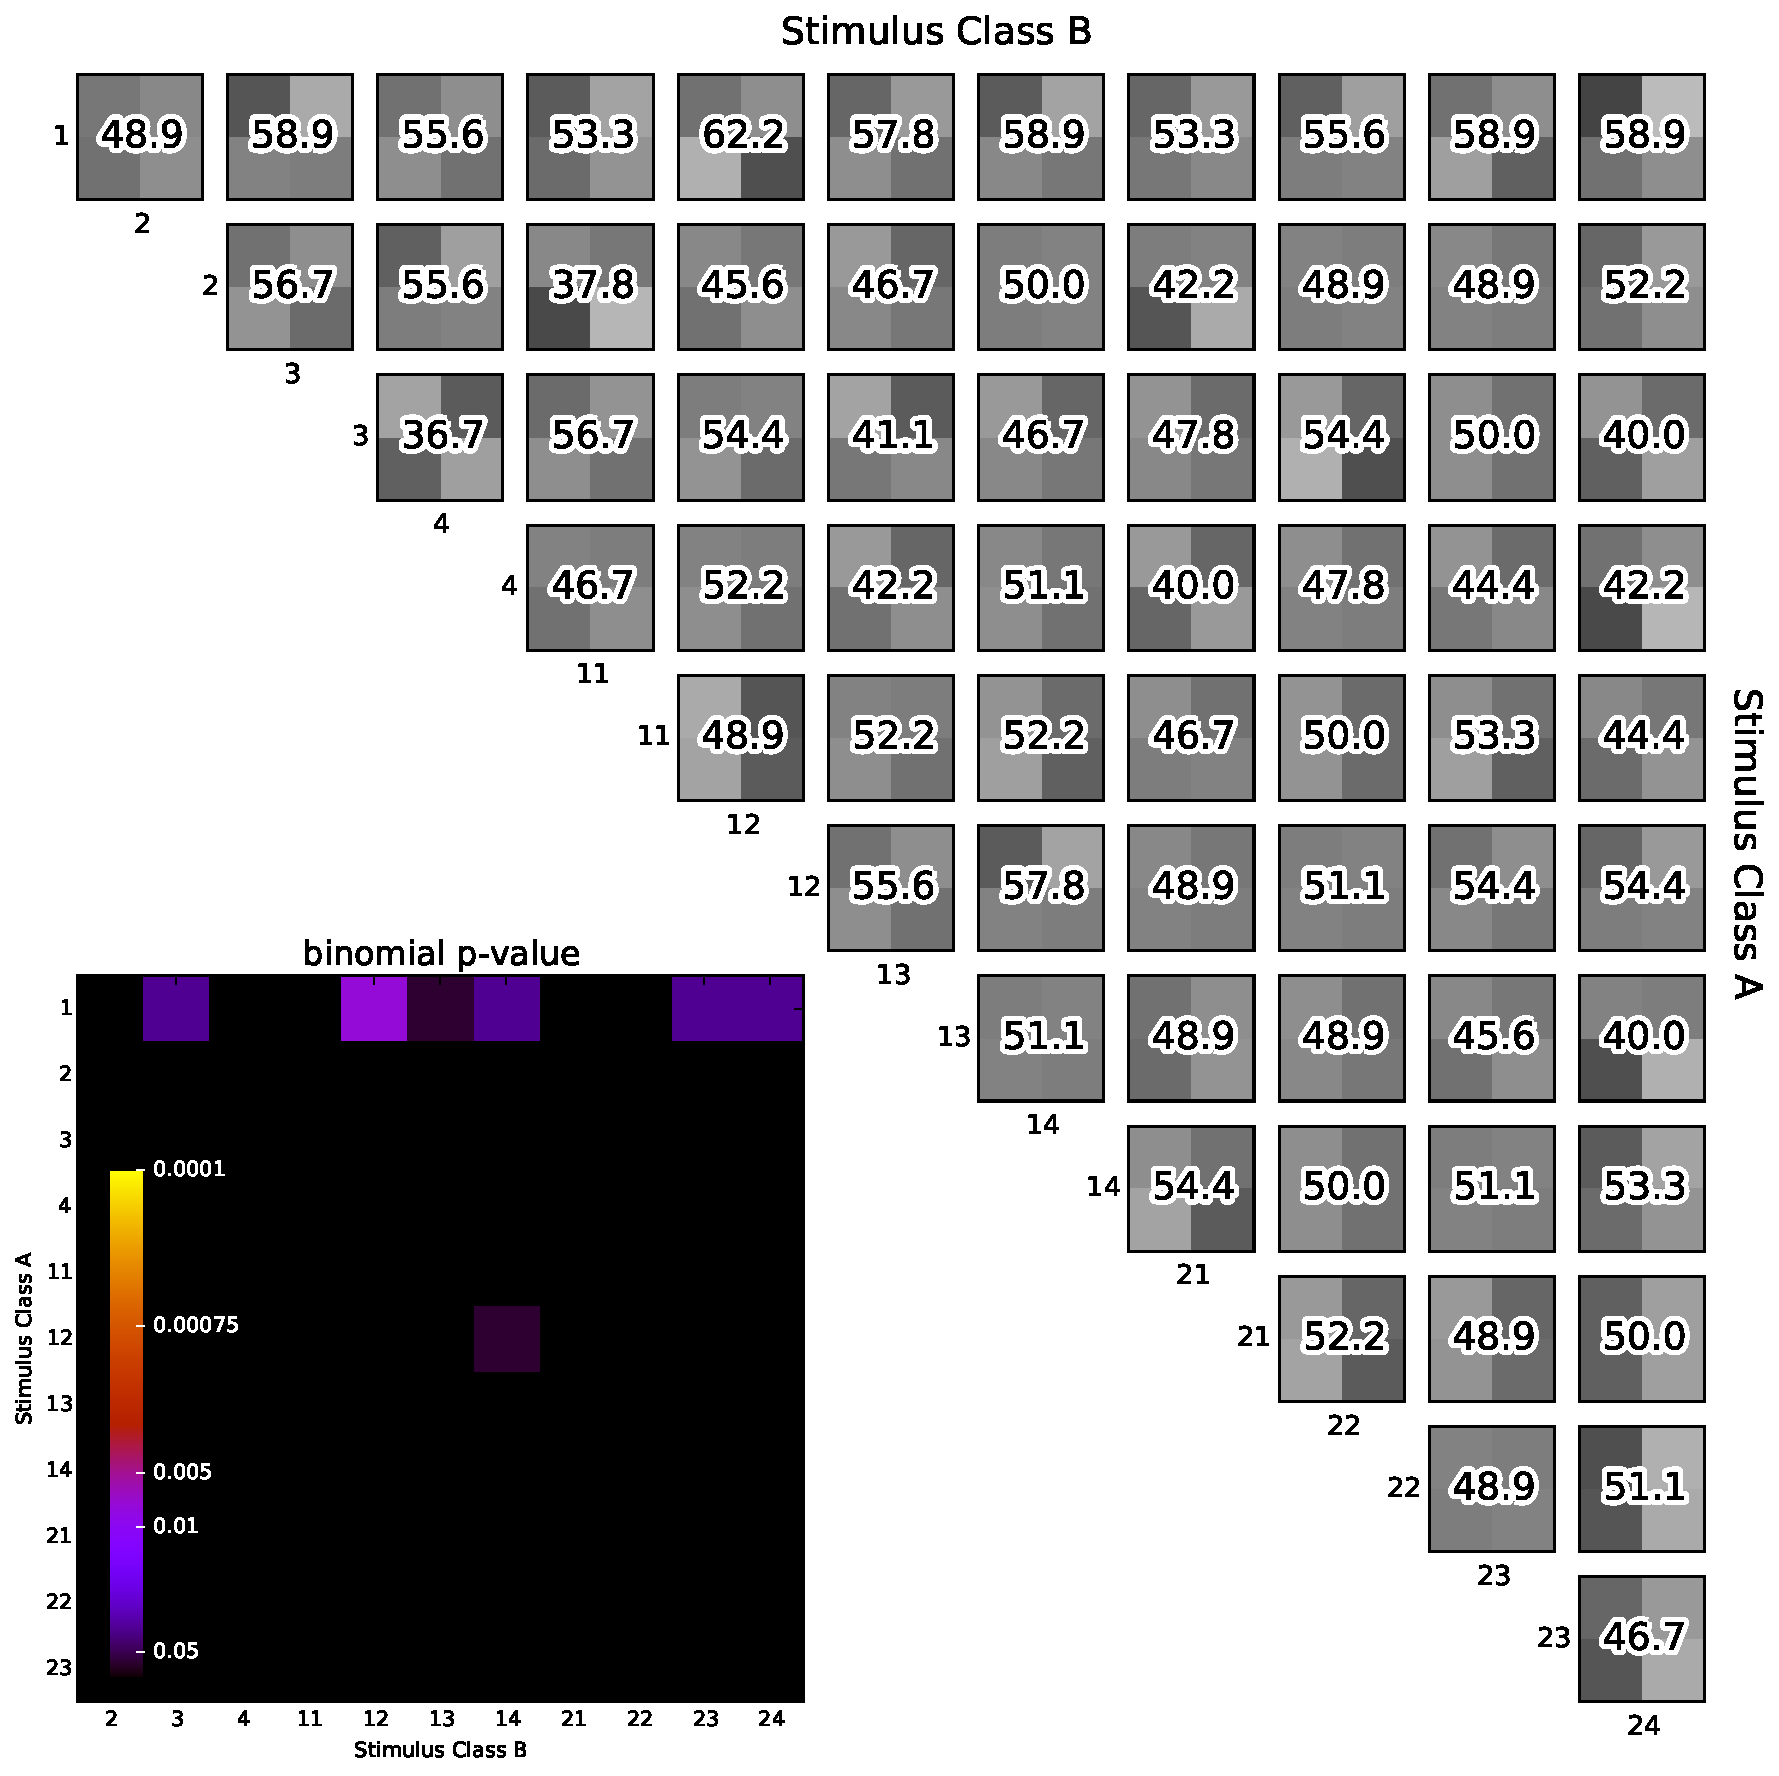
\includegraphics[width=.75\textwidth,keepaspectratio=true]{Figures/model_W_binary_confusion_cond2}
   \\\vspace{-0.8em}
    \caption{Binary confusion matrices for imagination data.
    The inset shows the p-values determined by using the cumulative binomial distribution to estimate the likelihood of observing the respective binary classification rate by chance. The significance threshold was bonferroni corrected to $alpha$ =  0.05/66 = 7.5e-04}
    \label{fig:model_W_binary_confusion_cond2}
  \end{center}
  \vspace{-1em}
\end{figure}
\newpage
\section{Discussion}
The neural net does not give us information about what characteristics from the EEG it used to classify the stimuli, and it is difficult to interpret from the results what signals the brain is producing that allow this classification to occur. 
In layer 3 of \autoref{fig:model_W} we see compressed representations of the EEG data for each stimulus. 
One characteristic of these representations is the dark red vertical bands that stand out from the rest of the time course. 
These red bands indicate time periods that the neural net has identified as being important for classifying the stimuli.
When taking a closer look, we see that these bands occur at the same time point for lyric/non-lyric pairs of stimuli. 
For example, the darkest red band in stimulus 1 (Chim Chim Cheree with lyrics) appears at a very similar time point as the darkest red band in stimulus 11 (Chim Chim Cheree without lyrics).
A similar pattern can be seen for stimuli 2/12 and 3/13.
Upon investigation of the audio of the stimuli at these time periods, there were no characteristics (e.g. lyric repetition, important music moments, end of phrases, change in dynamics, etc.) that stood out as driving these moments to be labeled as important.
These red bands may represent a cognitive process, such as recognition, that occurs at these time points during perception of the stimuli. 
To investigate this possibility, we ran a follow-up behavioural experiment asking participants to indicate when they consciously recognized each stimulus. 
This experiment is described in the next section.

The results of our neural net show that some stimuli are better classified than others, and some pairs of stimuli are more easily differentiated. 
To investigate whether the neural net is relying on a process similar to that which humans might employ, we ran a follow-up experiment asking participants to rate the similarity of pairs of stimuli. 
The results will tell us whether the neural net confuses songs that humans rate as similar. 